\documentclass{ltjsarticle}
% ltjsarticle: lualatex 用の 日本語 documentclass
% 他のタイプセットエンジンを使ってビルドする場合は、 \documentclass[dvipdfmx]{jsarticle} などとする。
\usepackage{graphicx}
\usepackage{mathrsfs}
\usepackage{amssymb}

\begin{document}

\title{Chapter 10 The Blahut-Arimoto Alogorithmes}
\author{Tetsuya SHIMIZU}
\maketitle

離散的無記憶通信路$p(y|x)$の場合,通信路容量は
\begin{eqnarray}
  \label{10.1}
  C = \max_{r(x)} I(X;Y)
\end{eqnarray}
となる.
ここで,$X$と$Y$はそれぞれ一般的な通信路の入力と出力,$r(x)$は入力分布であり,通信路をとおして情報を確実に伝送できる漸近的に達成可能な最大レートを特徴づける.
式(\ref{10.1})の$C$は,汎用通信路の遷移行列のみに依存し,通信路に対する符号のブロック長$n$には依存しないので,\textit{single-letter characterization}(一文字特性化)と呼ばれる.
入力アルファベット$\mathcal{X}$と出力アルファベット$\mathcal{Y}$の両方が有限であるとき,$C$の計算は有限次元の最大化問題となる.

一般的な確率変数$X$を持つi.i.d.情報源$\{X_k, k \geq 1\}$に対して,レート歪み関数
\begin{eqnarray}
  \label{10.2}
  R(D) = \min_{Q(\hat{x}|x): Ed(X,\hat{X}) \leq D} I(X;\hat{X})
\end{eqnarray}
1文字の歪み尺度$d$に関して$D$以下の平均歪みで情報源を再生するレート歪み符号の漸近的に達成できる最小レートを特徴付ける.
再び,式(\ref{10.2})の$R(D)$が一文字特性であり,これはレート歪み符号のブロック長$n$でゃなく,一般的な確率変数$X$だけに依存する.
情報源アルファベット$\mathcal{X}$と再生アルファベット$\hat{\mathcal{X}}$の両方が有限であるとき,$R(D)$の計算は有限次元の最小化問題となる.

よほど特殊な場合を除き,$C$や$R(D)$の式を閉じた形で得ることは不可能であり,数値計算に頼らざるを得ない.
しかし,これらの量を計算することは,関連する最適化問題が非線形であるため,一筋縄ではいかない.
本章では,このために考案された反復アルゴリズムであるBlahut-Arimotoアルゴリズム(以下,BAA)について解説する.

BAAがどのように,そしてなぜ機能するのかをよりよく理解するために,まず次のセクションで一般的な設定におけるアルゴリズムを説明する.
$C$と$R(D)$の計算のためのアルゴリズムの特殊化については2節で説明し,アルゴリズムの収束については3節で証明する.

\section{Alternating Optimization}
本節では,交互最適化アルゴリズムについて説明する.
このアルゴリズムは,次節で通信路容量とレート歪み関数を計算するために特化される予定である.
二重の$\sup$を考える.
\begin{eqnarray}
  \label{10.3}
  \sup_{\mathbf{u}_1 \in A_1} \sup_{\mathbf{u}_2 \in A_2} f(\mathbf{u}_1, \mathbf{u}_2)
\end{eqnarray}
ここで,$A_i$は$i = 1,2$について$\mathfrak{R}^{n_i}$の凸部分集合であり,$f$は$A_1 \times A_2$上で定義された関数である.
関数$f$は上方から有界であり,$A_1 \times A_2$上で連続的な偏導関数を持っている.
さらに,すべての$\mathbf{u}_2 \in A_2$に対して,
\begin{eqnarray}
  \label{10.4}
  f(c_1(\mathbf{u}_2), \mathbf{u}_2) = \max_{\mathbf{u}_1^{\prime} \in A_1} f(\mathbf{u}_1^{\prime}, \mathbf{u}_2)
\end{eqnarray}
を満たすような一意の$c_1 (\mathbf{u}_2) \in A_1$が存在し,すべての$\mathbf{u}_1 \in A_1$に対して,
\begin{eqnarray}
  \label{10.5}
  f(\mathbf{u}_1, c_2(\mathbf{u}_1)) = \max_{\mathbf{u}_2^{\prime} \in A_2} f(\mathbf{u}_1, \mathbf{u}_2^{\prime})
\end{eqnarray}
を満たすような一意の$c_2(\mathbf{u}_1) \in A_2$が存在するとする.

$\mathbf{u} = (\mathbf{u}_1, \mathbf{u}_2)$と$A = A_1 \times A_2$とすると,式(\ref{10.3})は式(\ref{10.6})と書くことができる.
\begin{eqnarray}
  \label{10.6}
  \sup_{\mathbf{u} \in A} f(\mathbf{u})
\end{eqnarray}

すなわち,$f$の$\sup$は,$\mathfrak{R}^{n_1}$と$\mathfrak{R}^{n_2}$の2つの凸部分集合のデカルト積に等しい$\mathfrak{R}^{n_1 + n_2}$の部分集合に対してそれぞれ取られる.

ここで,式(\ref{10.3})の二重$\sup$の値である$f^{*}$を計算するための交互最適化アルゴリズムについて説明する.
$k \geq 0$に対して$\mathbf{u}^{(k)} = ( \mathbf{u}_1^{(k)}, \mathbf{u}_2^{(k)} )$と定義する.
$A_1$において任意に選んだベクトルを$\mathbf{u}_1^{(0)}$と$\mathbf{u}_2^{(0)}=c_2 (\mathbf{u}_1^{(0)} )$する.
$k \geq 1$の場合,$\mathbf{u}^{(k)}$は
\begin{eqnarray}
  \label{10.7}
  \mathbf{u}_1^{(k)} = c_1 ( \mathbf{u}_2^{(k-1)} )
\end{eqnarray}
と
\begin{eqnarray}
  \label{10.8}
  \mathbf{u}_2^{(k)} = c_2 ( \mathbf{u}_1^{(k)} )
\end{eqnarray}
で定義される.
すなわち,$\mathbf{u}_1^{(k)}$,$\mathbf{u}_2^{(k)}$は,$A_1$において$\mathbf{u}_1^{(0)}$が任意に選ばれることを除いて,順序$\mathbf{u}_1^{(0)}, \mathbf{u}_2^{(0)}, \mathbf{u}_1^{(1)}, \mathbf{u}_2^{(1)}, \mathbf{u}_1^{(2)}, \mathbf{u}_2^{(2)}, \cdots$で生成され,順序の各ベクトルは前のベクトルの関数である.
\begin{eqnarray}
  \label{10.9}
  f^{(k)} = f( \mathbf{u}^{(k)})
\end{eqnarray}
とする.次に式(\ref{10.4})と式(\ref{10.5})から$k \geq 1$について
\begin{eqnarray}
  \label{10.10}
  f^{(k)} &=& f\left(\mathbf{u}_1^{(k)}, \mathbf{u}_2^{(k)}\right) \\
  \label{10.11}
  &\geq& f \left(\mathbf{u}_1^{(k)}, \mathbf{u}_2^{(k-1)}\right) \\
  \label{10.12} 
  &\geq& f \left(\mathbf{u}_1^{(k-1)}, \mathbf{u}_2^{(k-1)}\right) \\
  \label{10.13}
  &=& f^{(k-1)}
\end{eqnarray}
とする.
数列$f^{(k)}$は非減少であり,$f$は上から有界であるから収束するはずである.
3節で$f$が凹型であれば$f^{(k)} \rightarrow f^*$であることを示すことにする.
図\ref{fig10.1}は交互最大化アルゴリズムの説明図であり,この場合$n_1$も$n_2$も$1$に等しく,$f^{(k)} \rightarrow f^*$となる.
\begin{figure}[htbp]
  \label{fig10.1}
  \begin{center}
  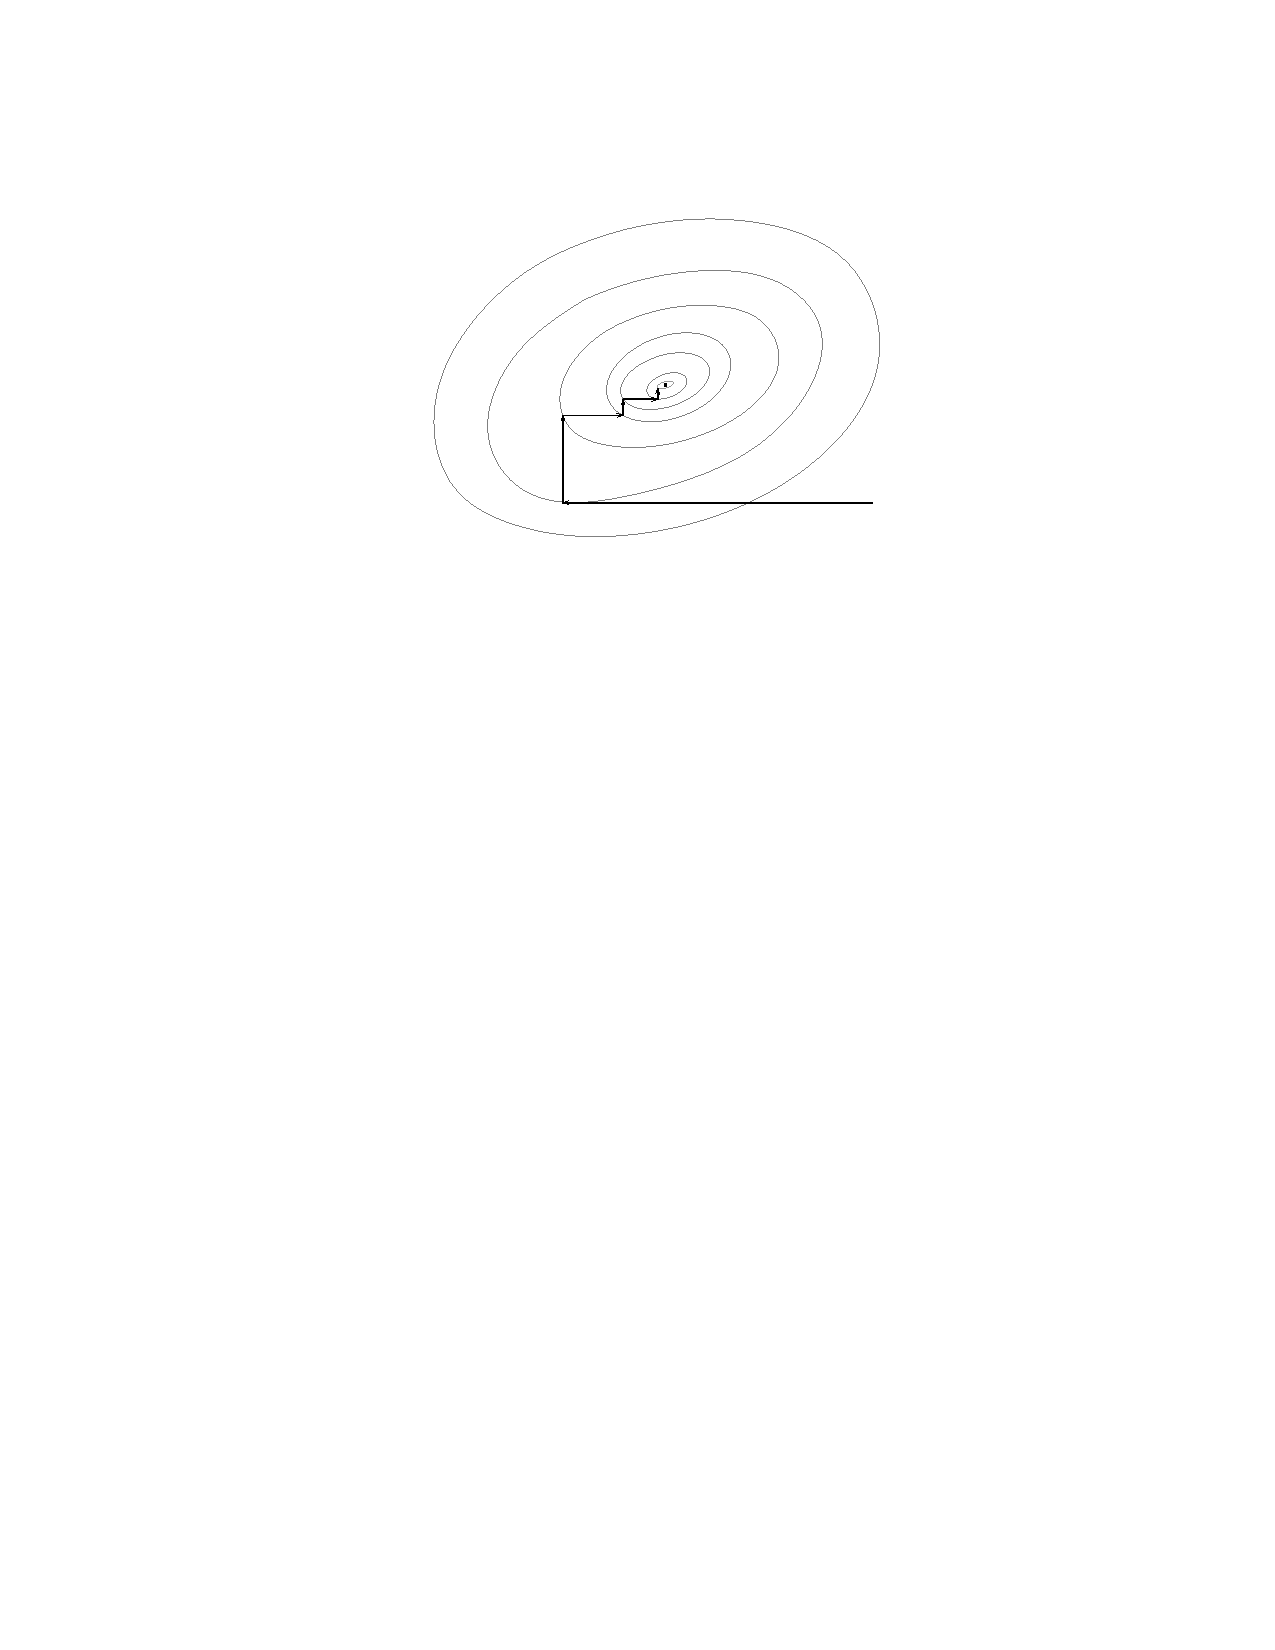
\includegraphics{Fig10-1.pdf}
  \caption{Alternating Optimization}
  \end{center}
\end{figure}

交互最適化アルゴリズムは,次のような系図で説明する事ができる.
あるハイカーが山頂を目指すとする.
山のある地点から出発して,南北と東西に交互に移動する.
(この問題では,南北と東西の方向は多次元的である.)
それぞれの移動で,ハイカーは可能な限り高い地点に移動する.
問題は,ハイカーが最終的に山のどの地点からでも山頂に近づくことができるかどうかである.

式(\ref{10.3})の$f$を$-f$に置き換えると,二重$\sup$は二重$\inf$を用いて
\begin{eqnarray}
  \label{10.14}
  \inf_{\mathbf{u}_1 \in A_1} \inf_{\mathbf{u}_2 \in A_2} f \left( \mathbf{u}_1, \mathbf{u}_2 \right)
\end{eqnarray}
となる.$A_1$,$A_2$,$f$に関するこれまでの仮定は,$f$が上方から有界でなく下方から有界であることを仮定した以外はすべて有効である.
式(\ref{10.14})の二重$\inf$は,同じ交互最適化アルゴリズムで計算することができる.
なお,$f$を$-f$に置き換えると,式(\ref{10.4})と式(\ref{10.5})の最大値は最小値になり,式(\ref{10.11})と式(\ref{10.12})の不等号は逆になる.

\end{document}